\chapter{Survival analysis} \label{ch:surv}
\section{Methods}
The time series approaches provide a good prediction on turnover based on organizational level. However, more questions are brought to the forefront, like when a specific employee will turnover, what factors affect employee's turnover, why they will turnover: voluntary quit, retire, or by other reasons. And also the dataset has two kinds of unknown information. There are active employees who are hired from November 1st, 2000 to July 12th, 2012, and terminative employees who left the organization from November 1st, 2000 to July 12th in the dataset. The turnover date for active employees who left after July 12, 2012 and the information for terminative employee who left before November 1st, 2000 are both not available. These two kinds of  unknown information cause two kinds of bias: right censoring and left truncation. Besides, there is an intervention event implemented by HR in 2008 which is a downsizing policy to incent the employees who are eligible for retirement to retire. Therefore, how to model this incentive and to estimate its effect are another interesting questions. All these questions and problems can be solved by lifetime analysis, also called survival analysis. The cox proportional hazard model is to build the forecasting model, to generate a base line, and to identify significant factors for turnover. Competing risks analysis is used to answer what kind of reasons cause employees  turnover. A time dependent covariates is created for year 2008 to model the incentive effect and to achieve more accurate forecasting result. Finally, a simulation study is performed to examine the forecasting capability of cox proportional hazard model on the left truncation and right censor dataset.
\subsection{Right censoring and left truncation}
Right censoring and left truncation are common in survival analysis. The right censoring is that the main event of interest (failure) occurs after the study window. Let $T$ denotes the time of main event of interest to occur and let $C$ denotes the end time of study. An observation is right censored when $T> C$, indicating the study do not have the failure time of the right censored observation. In this study, the study window is from November 1st, 2000 to July 12th, 2012. Thus, employees who leave the organization after the study window are right censored. These right censored observations require special treatment in survival analysis: a censor indicator variable is created: 
\begin{align*}
\delta_i&=
\begin{cases}
1   &\text{if  }  t_i \leq c_i \text{ (uncensored),}\\
0   &\text{if  }  t_i > c_i \text{ (censored),}
\end{cases}
\end{align*}
where, $i$ denotes the ith observation, and the failure time of event for ith observation is minimum time between $t_i$ and $c_i$, i.e., $min(t_i, c_i)$, that is when $ c_i <t_i $, $c_i$ is taken as end time of the ith observation in order to do next  analysis.

Left truncation is that the occurrence of an intermediate event prior to the main event of interest appear in the sample dataset. Left truncation in this study occurs when employees enter to the organization at random time, that is, the hired time precedes the origin of the study window. Then, the employees are followed from this entry time until the turnover events occur or until they are right-censored. So, the employees turnover before the entry time of the study will not be aware or not be in the sample dataset. Let $T$ denotes the time of main event of interest to occur and let $X$ denotes the time an individual enters the study, that is time of truncation events occurs. Only the individuals with $T \geq X$ are observed in the study window. The left truncation leads to the bias in the analysis. For example, employees who entered the company in 1950s, appear to stay longer as compared the employees entered in 1960s or later, causing by the fact that the sample dataset does not include the observation recorders for the employees who left the organization before November, 2000. The existence of truncation in the data must be taken into account in order to overcome this bias and to achieve accurate estimation of survival analysis \citep{carrion2010}. Let $t_{i0}$ denotes the start time of the ith observation, i.e., hired time or age at hired of ith employee, $x_{i}$ denotes the entry time of the ith observation, i.e., the start time of study (November 1st, 2000) or age at November 1st, 2000. The start time of the observation is maximum value between $t_{i0}$ and $x_i$, that is when $t_{i0} < x_i $, $x_i$ is taken as start time of the ith observation in order to eliminate the left truncation bias \citep{allison1995}. The number of failures in the $t_j$ is redefined for left truncation. When $x_i < t_j \le t_i$, the observation is in the risk set. When $t_{j} < x_i \le t_i$, the ith observation has not entered study yet at $t_j$ and it cannot be considered in the risk set. When $x_i \le t_i < t_j$, it indicates the ith observation whose failure time before $t_j$, and it cannot be considered in the risk set at time $t_j$ neither \citep{carrion2010}.
%%%%%%%%%%%%%%%%%%%%%%%%
%%%%%%%%%%%%%%%%%%%%%%%%
%%%%%%%%%%%%%%%%%%%%%%%%

\subsection{Cox proportional hazard regression}
Cox proportional hazards regression is a widely used method for estimating survival distributions. It was introduced in a seminal paper by \citet{cox1972}. The Cox PH model is usually taken the form of hazard model formula shown \ref{eq:cox}:
\begin{equation}
\label{eq:cox}
h(t,x)=h_0(t)e^{(\sum_{i=1}^{k}\beta_ix_i)}
\end{equation}

where $x=(x_1, x_2, \ldots, x_k)$, $h_0(t)$ is the baseline hazard occurring when X=0, $\beta$ is the coefficients of $x$. 
The model provides a hazard expression at time t for an individual with a given specification of a set of explanatory variables denoted by the $x$. The Cox PH formula is the product of quantities at hazard time $t$: $h_0 (t)$ as the baseline hazard function and the exponential expression to the linear sum of $\beta_i x_i$, where the sum is over the $k$ explanatory $X$ variables. $x$ can be time-independent covariates, because it does not involve time $t$, or time-dependent covariates which Cox PH model is called the extended Cox model. Because the baseline hazard function $h_0 (t)$ is an unspecified function, the Cox PH model is a semiparameric model, whose estimation can closely approximate correct parametric model \citep{kleinbaum1998}, causing the semiparameric model is "robust" and popular. Taking the logarithm of both sides of the equation, the Cox PH model is rewritten in equation \ref{eq:coxlog}:
\begin{equation}
\label{eq:coxlog}
\log{h(t,x)}=\alpha(t)+\sum_{i=1}^{k}\beta_ix_i 
\end{equation}
where $\alpha(t)=\log{h_0(t)}$. If $\alpha(t)=\alpha$, the baseline is exponential distribution and the model is exponential model. In Cox PH model, $\alpha(t)$ do not limited on specific parametric distributions and it can take any form. The partial likelihood method is used to estimated $\beta$ coefficients of the Cox model without having to specify the baseline \citep{allison1995}.
%%%%%%%%%%%%%%%%%%%%%%%%
%%%%%%Time dependent %%%%%%%%%%
%%%%%%%%%%%%%%%%%%%%%%%%
\subsection{Time dependent covariate}
Time dependent covariate depicts that a covariate is not necessarily constant through the whole study and change values over the course of the observation. The extended Cox model incorporates both time-independent and time-dependent covariates as shown in equation \ref{eq:timecovar}:
\begin{equation}
\label{eq:timecovar}
h(t,x)=h_0(t)e^{(\sum_{i=1}^{k_1}\beta_ix_i+\sum_{j=1}^{k_2}\gamma_jx_j(t))}
\end{equation}
where $x=(x_1, x_2, \ldots, x_{k_1}, x_1(t), x_2(t), \ldots, x_{k_2}(t))$, $h_0(t)$ is the baseline hazard occurring when $x=0$, $\beta$ and $\gamma$ are the coefficients of $x$. 
%%%%%%%%%%%%%%%%%%%%%%%%
%%%%%%Competing risk analysis%%%%%%%%
%%%%%%%%%%%%%%%%%%%%%%%%
\subsection{Competing risks analysis}
A competing risk is an event whose occurrence either precludes the occurrence of the event of interest or fundamentally alters the probability of occurrence of this event of interest \citep{tableman2003}. For example, turnover causes of an employee are exclusive and independent, i.e. an employee can experience only one event such as voluntary quit rather than retirement. This alters the probability of experiencing the event of interest, like retirement. Such events are known as competing risks events where one event of several different types of possible events can occur and hence the survival analysis for each event is calculated separately with the other events set as censored. Two mutually exclusive causes are considered as the event of interests for each employees in this study, which are voluntary quit and retirement. And the other events are treat as censored.

The reason for studying retirement and voluntary quit is because the organization are interested in forecasting the turnover of retirement of voluntary quit. There are $1/3$  employees in that organization are over 50 years old who are eligible for retirement. The employee for voluntary quit usually is the one organization would not like to leave \citep{allen2010}. And voluntary quit costs highly for the organizations and firms \citep{selden2000}. The other reasons of turnover, such as layoff, transfer, death, or disability are not considered, because the factors causing the occurrence of these turnover are random and hard to predict. The Cox PH models for competing risks as shown in equation \ref{eq:competing}:
\begin{equation}
\label{eq:competing}
h_j(t,x)=h_{j0}(t)e^{(\sum_{i=1}^{k}\beta_{ij}x_i)}
\end{equation}
where, $x_{j}$ is the covariate for a specific type of turnover. Note that the coefficient $\beta$ is the effects of the covariates may be different from different turnover types. If $\beta_{ij}$  is the same for all j, the model simplified to Cox PH model as shown in equation \ref{eq:cox}. 
%%%%%%%%%%%%%%%%%%%%%%%%%%%
%   Data preparation
%%%%%%%%%%%%%%%%%%%%%%%%%%
\subsection{Data preparation}
The dataset is split into two datasets by time point November 1st 2010: training and holdout. The training part is used to build the model (November 1st, 2000 - October 31th, 2010), and the holdout part is to validate the model performance (November 1st, 2010 - July 12, 2012). Age of employees is used to build the model as dependent variable rather than the length of service time in the organization. The age is calculated based on two time points: start age and leaving age. Start age is the age of an employee at hired in the organization, or the age at November 1st 2000, when the employee was hired before November 1st, 2000; leaving age is the age at the date who left the organization or the age at October 31st 2010, if the employee was still working in the organization at that time which are treated as censored data. The covariates identified from the turnover dataset and used to build the final model are payroll, gender, organization level, cocs code, age at hired, year of service at hired, termination date and termination type: 
\begin{itemize}
	
	\item Payroll (PR): hourly, weekly, or monthly payroll, 
	\item COCS code: Crafts(C), Engineers (E), General Administrative (G), Laborers (L), General Managers (M),  Administrative (P),  Operators (O), Scientists (S), Technicians (T))
	\item Gender: male, female
	\item Age at hired: most recent age when an employee is hired.
	\item Age at started: the age of an employee at November, 2000, if employee hired before November, 2000, or the age of an employee at hired, if employee hired after November, 2000. 
	
	\item Years of service at hired (YCSH): the years of service which accounts for pension plan when employee is most recently hired.
	\item Termination date: the date when an employee left the organization.
	\item Termination type: the reasons for employees leaving the organization, such as retirement(RE),  volunteer quit (VQ), and other reasons. 
	\item Age at end: the age of an employee at termination date, if employee left the organization before October 31th, 2010, or the age of an employee at October 31th, 2010.
	\item Organization level (ORG): the divisions of the organization.
\end{itemize}
A time-dependent covariate (policy) is created to model the incentive for 2008. Time dependent covariate is a dummy variable:
\begin{align*}
Policy&=
\begin{cases}
1   &\text{if employee works in year 2008 }\\
0   &\text{if  employee does not work in year 2008}
\end{cases}
\end{align*}
%%%%%%%%%%%%%%%%%%%%%%%%
%%%Model evaluation and variable selection%%%%
%%%%%%%%%%%%%%%%%%%%%%%%

\subsection{Model evaluation and variable selection}
The training dataset is applied to Cox PH model to build employee working lifetime distribution utilizing individual demographic information. Then the coefficients of covariates and the baseline from the model are used to calculated the turnover probability for each employee as shown in equation \ref{eq:prob}. 
\begin{equation}
\label{eq:prob}
\begin{split}% to allgin the equation
P\{t_{j-1}<T<t_j\} &=1-P\{T>t_j|T \ge t_j\}\\
&=1-\frac{S_{t_j}}{S_{t_{j-1}}}   \\
&=1-\frac{{S_0(t_j)}^{(\sum_{i=1}^{k}\beta_ix_i)}}{   {S_0(t_{j-1})}^{(\sum_{i=1}^{k}\beta_ix_i)}}
\end{split}
\end{equation}
where, $T$ is survival time, $t_j$ is a specific value for $T$, $S_0(t)$ is the baseline function generated by Cox PH model, $x$ is the covariates, and $\beta$ is the coefficient.
The expected turnover number is achieved by the summation of turnover probability for all the active employees at $t_j$ as shown in \ref{eq:expturnover}.  
\begin{equation}
\label{eq:expturnover}
E(\text{turnover number at } t_j)=\sum_{i=1}^k{P_i\{t_{j-1}<T<t_j\}} 
\end{equation}
where, $i$ denotes the ith observation. -2 log likelihood statistic, Akaike’s information (AIC) and Schwartz’s Bayesian criterion (SBC) are applied to evaluate model performance and select variables. The variable selection procedure is manually backwards selection. First, put all the variables into the model. Second, remove one non-significant variable ($P>0.05$) and rerun the model again to compare AIC and SBC value with those value of previous model. If there is no or very small difference between current and previous model, the model selection stops and the variables in the model are selected variables. Otherwise, repeat the second step. The evaluation step is to calculate the yearly predicted turnover number for training and holdout dataset, and then compared the predicted number with the actual number. The survival analysis is performed on software SAS and R package.
%add evaluation formula.
%%%%%%%%%%%%%%%%%%%%%%%%
%%%Simulation on left truncation and right censor%%%%
%%%%%%%%%%%%%%%%%%%%%%%%
\subsection{Simulation on left truncation and right censor}
The simulation is used to examine Cox PH model predictive performance with right censoring and left truncation. The generation  of simulation lifetime data is based on the Weibull distribution. %The hazarld function for Weibull regression model with shape parameter $\alpha$, scale parameter $\lambda$, and covariate $X$ is shown in equation \ref{eq:weibul}, given $h_0=\alpha(\lambda)^\alpha t^{\alpha-1}$: 
%\begin{equation} \label{eq:weibul}
%\begin{split}% to allgin the equation
%h(t|X) & =h_0(t)exp(\beta X) \\
%         &=\alpha (\lambda (exp(\beta X)^{\frac{1}{\alpha}})^\alpha t^{\alpha-1} \\
%         &=\alpha(\tilde{\lambda} )^\alpha t^{\alpha-1}
%\end{split}
%\end{equation}
%where, $\tilde{\lambda}=\lambda (exp(\beta X)^{\frac{1}{\alpha}}$.
The simulation can be described as follows. The sample size was n=4000, with one variable $X$, named Age, which follows uniform distribution with parameter $a$ $(a=22)$ and $b$ $(b=70)$. Only one variable age is used in simulation process to make the estimation procedure simple and close to real world. The coefficient $\beta_{age}$ is taken $-0.025$ and $\beta_0=1.5$. 
Then, the survival time $T$ is random generated for each observation based on Weibull distribution with shape parameter $\alpha$ and scale parameter $\lambda$, where $\alpha=1.5$ and $\lambda=exp(-0.025age+\beta_0)^{\frac{1}{\alpha}}$.

The simulation is performed on right censoring and left truncation separately, in order to observe the effects for different bias.  
For right censoring simulation, the start point for all the observations are set as 0, and stop point is equal to the survival time $t_i$ for ith observation where $T=(t_1, t_2, \ldots, t_n)$. After that, a survival time histogram is generated. The censor time $C$ is set as first quarter, median, third quarter, and maximum of the survival time, respectively, to get 75\%, 50\%, 25\% and 0\% censoring proportions. When the survival time $t_i$ for ith observation is not greater than the censor time ($c_i$), the stop point is survival time and censor variable $\delta_i$ is 1. When survival time $t_i$ for ith observation is greater than censor time ($c_i$), the stop point is change to censor time ($c_i$) and censor variable $\delta_i$ is  0. The start point and the stop point are dependent variable in the cox regression model. $\delta$ is censor variable. And variable age is predictor or covariate. All these variables are applied to cox model using R EHA package. 

For left truncation simulation, the start point $U$ is generated as uniform distribution with $a=0$ and $b=max(T)$ which indicates an observation start randomly from time 0 to time $max(T)$. The stop point $S$ is $U+T$. The histogram is generated for $S$. The truncation time $L$ is set as 0, first quarter, median, and third quarter of $S$, respectively, to get 0\%, 25\%, 50\%, and 75\% truncation proportions. When start point $u_i$ for ith observation is less than truncation time $l_i$, the start point is reset as truncation time $l_i$. When start point $u_i$ for ith observation is not less than truncation time $l_i$, the start point does not change ($u_i$). In left truncation, the censor variable $\delta$ for all the observations are equal 1. All these variables are also used to build Cox PH model in R EHA package. The Cox PH model is conducted using "phreg" function in eha package and using weibull distribution to estimate the baseline for both right censoring and left truncation simulation. The "phreg" function performs Cox PH model and also provides a parametric baseline hazards estimation \citep{brostrom2012}. Total predicted failure number is calculated as shown in equation \ref{eq:prob} and \ref {eq:expturnover}. The actual and forecast failure number are plotted to compare the effects on different levels of bias.

%accelarate model%

%%%%%%%%%%%%%%%%%%%%%%%%%%%
%%%%%%%%%%%%%%%%%%%%%%%%%%%
%%%                           Result              %%%%%%%%%%
%%%%%%%%%%%%%%%%%%%%%%%%%%%%


%%%%%%%%%%%%%%%%%%%%%%%%%%%
%%%%%%%%%%%%%%%%%%%%%%%%%%%
%%%                       Simulation   Result              %%%%%%
%%%%%%%%%%%%%%%%%%%%%%%%%%%
\section{Survival analysis results}
\subsection{Cox PH Model Analysis Result without Time-dependent Covariate}
A turnover model for entire organization is built by survival analysis.  Table \ref{tab:fit1} indicates that the accuracy of cox model fit is improved after adding covariates, as the -2 log Likelihood value, AIC and SBC value decrease with covariates. The model is statistically significant as all the p-values are less than 0.05 with 19 degrees of freedom. Table \ref{tab:variable1} shows the variables: payroll(PR), organization level (ORG), COCS code, age at start, and year of service at hired (YCSH) are statistically significant and cannot be eliminated from the model due to significant p-values. The test has nine degrees of freedom (df), corresponding to the nine coefficients that are estimated for ORG and six degrees of freedom corresponding to the six coefficients that are estimated for COCS. This test is the overall test for each variable which is omitted the category. Table \ref{tab:para1} shows the parameter estimates and the hazard ratio for each variable. Parameter estimates shows the coefficients estimates and associated statistics. Notice that there is no intercept estimate in Cox PH model. There are eight lines for the COCS variable. The first six lines contain coefficients, standard errors, and hypothesis tests for level 1 to level 6 of COCS, while the last two lines informs us that level 7 and level 8 are the omitted category. Hence, each of the estimated coefficients is a contrast with reference group of level 9. For categorical variables, the hazard ratio is the ratio of the current group to the reference group, which almost exactly like odds ratio in logistic regression. The hazard ratio for payroll 1 (monthly payroll) is 0.71, indicating that the hazard of leaving the organization for those with monthly payroll is only about 71 percent of the hazard for those with hourly payroll ( adjusted with other covariates). For the continuous variable like Age at start, the hazard ratio is 0.81, which yields 100(0.81-1)=-19, indicating that for each 1-year increase in the age at start for an employee, the hazard of leaving goes down by an estimated 19\%. The different hazard ratios for ORG levels indicate the different turnover behaviors among organization level. The different hazard ratios for COCS indicate the different turnover behaviors among different job classification. Besides, the hazard ratios of Age at start, YCSH are all less than 1, indicating that an employee hired with certain age and years of service are less likely to leave the organization than a new employee with young age and 0 years of service.
\begin{table}[htbp]
	\small
	\centering
	\caption{Model Fit Statistics}
	\begin{tabular}{rrr}
		\hline
		\multicolumn{1}{c}{Criterion} & \multicolumn{1}{c}{Without Covariates} & \multicolumn{1}{c}{With Covariates} \\
		\hline
		-2 LOG L & \multicolumn{1}{c}{46130.96} & \multicolumn{1}{c}{41978.58} \\
		AIC   & \multicolumn{1}{c}{46130.96} & \multicolumn{1}{c}{42016.58} \\
		SBC   & \multicolumn{1}{c}{46130.96} & \multicolumn{1}{c}{42132.62} \\
		\hline
	\end{tabular}%
	\label{tab:fit1}
\end{table}%

% Table generated by Excel2LaTeX from sheet 'Sheet2'
\begin{table}[htbp]
	\small
	\centering
	\caption{Variables Statistics Test}
	\begin{tabular}{cccc}
		\hline
		Effect & DF    & Wald $\chi^2$ &  Pr>$\chi^2$ \\
		\hline
		PR    & 2     & 9.2717 & 0.0097 \\
		ORG   & 9     & 1930.686 & $<.0001$ \\
		COCS  & 6     & 25.0608 & 0.0003 \\
		Age at start  & 1     & 673.0102 & $<.0001$ \\
		YCSH  & 1     & 640.4862 &$ <.0001$ \\
		\hline
	\end{tabular}%
	\label{tab:variable1}
\end{table}%
% Table generated by Excel2LaTeX from sheet 'Sheet2'
\begin{table}
	\centering
	\small
	\caption{Cox PH model parameter estimates}
	\begin{tabular}{cccccccc}
		\hline
		Parameter & Label & DF    &  Estimates & Std. Error & $\chi^2$    &  $Pr>\chi^2$ & Hazard Ratio \\
		\hline
		PR    & PR 1  & 1     & -0.346 & 0.134 & 6.64  & 0.01  & 0.71 \\
		PR    & PR 2  & 1     & -0.226 & 0.095 & 5.71  & 0.02  & 0.80 \\
		ORG   & ORG 1 & 1     & 3.465 & 0.381 & 82.77 & $<.0001$ & 31.98 \\
		ORG   & ORG 2 & 1     & 2.464 & 0.383 & 41.50 & $<.0001$ & 11.75 \\
		ORG   & ORG 3 & 1     & 2.012 & 0.393 & 26.21 & $<.0001$ & 7.48 \\
		ORG   & ORG 4 & 1     & 2.203 & 0.385 & 32.69 & $<.0001 $& 9.06 \\
		ORG   & ORG 5 & 1     & 2.378 & 0.399 & 35.53 & $<.0001$ & 10.78 \\
		ORG   & ORG 6 & 1     & 2.302 & 0.397 & 33.58 & $<.0001$ & 9.99 \\
		ORG   & ORG 7 & 1     & 4.461 & 0.381 & 137.28 & $<.0001$ & 86.60 \\
		ORG   & ORG 8 & 1     & 4.628 & 0.384 & 145.23 & $<.0001$ & 102.28 \\
		ORG   & ORG 9 & 1     & 3.780 & 0.383 & 97.69 & $<.0001$ & 43.83 \\
		Cocs  & Cocs 1 & 1     & -0.041 & 0.074 & 0.30  & 0.59  & 0.96 \\
		Cocs  & Cocs 2 & 1     & 0.194 & 0.126 & 2.37  & 0.12  & 1.22 \\
		Cocs  & Cocs 3 & 1     & -0.011 & 0.095 & 0.01  & 0.91  & 0.99 \\
		Cocs  & Cocs 4 & 1     & 0.117 & 0.086 & 1.85  & 0.17  & 1.12 \\
		Cocs  & Cocs 5 & 1     & 0.018 & 0.126 & 0.02  & 0.89  & 1.02 \\
		Cocs  & Cocs 6 & 1     & -0.101 & 0.123 & 0.67  & 0.41  & 0.90 \\
		Cocs  & Cocs 7 & 0     & 0.000 & .     & .     & .     & . \\
		Cocs  & Cocs 8 & 0     & 0.000 & .     & .     & .     & . \\
		Age at start  &       & 1     & -0.208 & 0.008 & 673.01 & $<.0001$ & 0.81 \\
		YCSH  &       & 1     & -0.069 & 0.003 & 640.49 & $<.0001$ & 0.93 \\
		\hline
	\end{tabular}%
	\label{tab:para1}
\end{table}%


\begin{figure}[htbp]
	\centering
	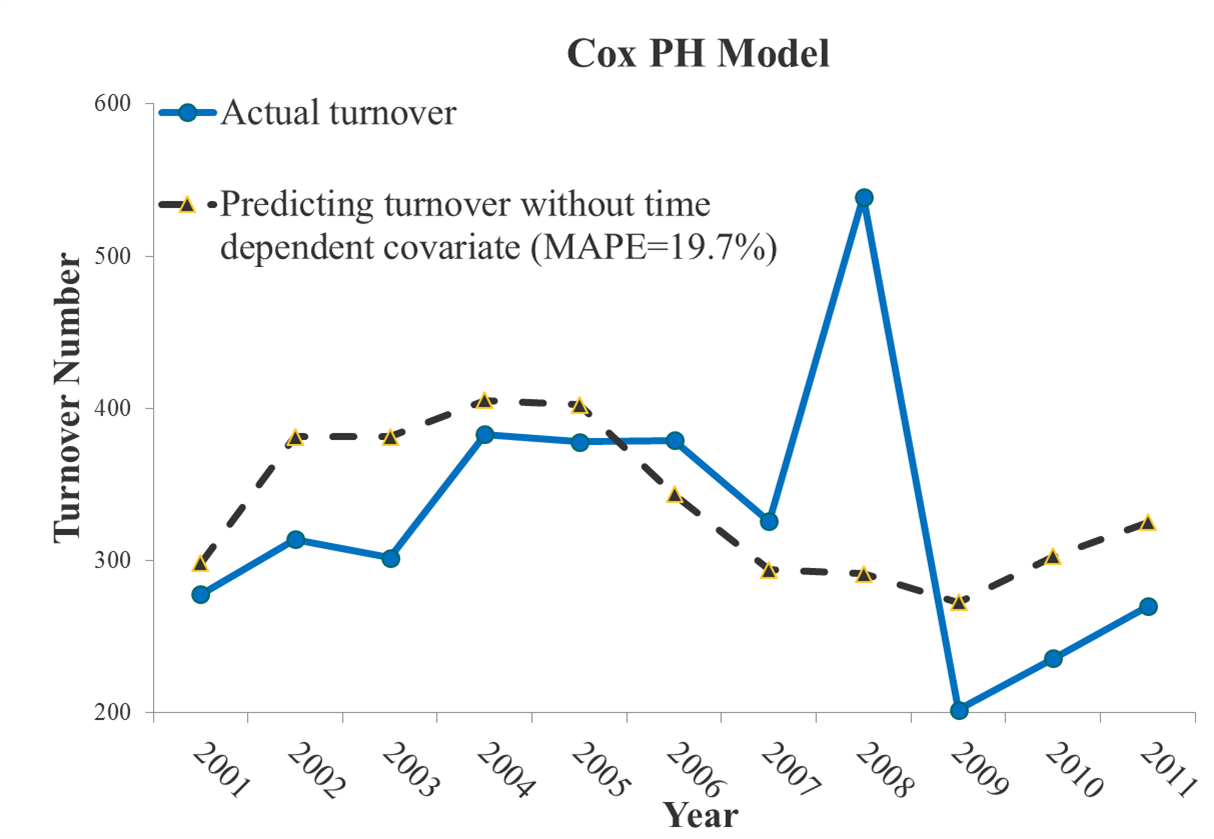
\includegraphics[width=5.5in]{Fig8.png}
	\caption{Actual vs. predicted turnover number for Cox PH model}
	\label{fig:8}
\end{figure}
All the data including training and holdout dataset are calculated the expected turnover number. The data for 2011 is holdout data set. The model performance as shown in Figure \ref{fig:8} is reasonable for the time period between 2004 and 2007 as the variation between them is quite insignificant. The model underestimates 2008 and overestimates after 2008 onwards. Year 2008 turnover number is much larger than the other years, because of an incentive policy published in that year leading to an increase in employee turnover in that year.  A new model with time-dependent covariates  has to be considered to accommodate the intervention event of year 2008.
%%%%%%%%%%%%%%%%%%%%%%%%%%%%
%%%%%%%%%%%%%%%%%%%%%%%%%%%%%%%%
%%%%%%%%%%%%%%%%%%%%%%%%%%%%%%%%
%%%%%%%%%%%%%%%%%%%%%%%%%%%%%%%%
\subsection{Cox PH Model with Time-dependent Covariate}
A time-dependent covariate (policy) is applied to model the intervention for 2008. It is a significant difference for AIC values before and after policy adding into the model and also the p-value is less than 0.05. Therefore the policy cannot be removed from the model. The variables: Payroll, ORG, YCSH, Age at Start all make a significant difference for the model without covariates and also statistically significant due to small p-values. Thus, they are all applied into the model. However, the variable COCS and Gender are not statistically significant due to the p-value larger than 0.05. These two variables can be removed from the model. Table \ref{tab:fit2} shows the model is statistically significant and Table \ref{tab:var2} indicates all the variables:  Policy, PR (payroll), YCSH (years of service at hired), ORG (organization level) and Age at start) are statistically significant with p-value less than 0.05. Table \ref{tab:para2} shows the parameter estimates and statistics for Cox PH model with variable policy. The hazard ratio for policy$=1$ is 3.18 indicating that the hazard of employees leaving the organization with an incentive policy is only about 318\% percent of the hazard without the incentive policy (adjusted with other covariates). After plotting the actual and predicted turnover number, the intervention is captured by the adjusted model in 2008 as clearly shown in the Figure \ref{fig:9}. Therefore, this model preforms better than the model without time-dependent covariate.  

% Table generated by Excel2LaTeX from sheet 'w time-covar'
\begin{table}[htbp]
	\small
	\centering
	\caption{Model Fit Statistics}
	\begin{tabular}{rrr}
		\hline
		\multicolumn{1}{c}{Criterion} & \multicolumn{1}{c}{Without Covariates} & \multicolumn{1}{c}{With Covariates} \\
		\hline
		-2 LOG L & \multicolumn{1}{c}{45729.81} & \multicolumn{1}{c}{41251.60} \\
		AIC   & \multicolumn{1}{c}{45729.81} & \multicolumn{1}{c}{41279.60} \\
		SBC   & \multicolumn{1}{c}{45729.81} & \multicolumn{1}{c}{41364.99} \\
		\hline
	\end{tabular}%
	\label{tab:fit2}%
\end{table}%

% Table generated by Excel2LaTeX from sheet 'w time-covar'
\begin{table}[htbp]
	\small
	\centering
	\caption{Variables Statistics Test}
	\begin{tabular}{cccc}
		\hline
		Effect & DF    & Wald $\chi^2$ &  $Pr>\chi^2$ \\
		\hline
		ORG   & 9     & 2075.926 & $<.0001$ \\
		YCSH  & 1     & 663.0154 & $<.0001$ \\
		PR    & 2     & 46.7408 & $<.0001$ \\
		Policy & 1     & 380.682 & $<.0001$ \\
		Age at start  & 1     & 457.5078 & $<.0001$ \\
		\hline
	\end{tabular}%
	\label{tab:var2}%
\end{table}%

% Table generated by Excel2LaTeX from sheet 'w time-covar'
\begin{table}[htbp]
	\small
	\centering
	\caption{Cox PH Model Parameter Estimates with Variable Policy}
	\begin{tabular}{cccccccc}
		\hline
		Parameter & Label & DF    &  Estimate & Std. Error & $\chi^2$    & $ Pr>\chi^2$ & Hazard Ratio \\
		\hline
		ORG   & ORG 2 & 1     & -0.989 & 0.073 & 185.051 & $<.0001$ & 0.372 \\
		ORG   & ORG 3 & 1     & -1.369 & 0.115 & 141.977 & $<.0001$ & 0.254 \\
		ORG   & ORG 4 & 1     & -1.244 & 0.086 & 210.286 & $<.0001$ & 0.288 \\
		ORG   & ORG 5 & 1     & -1.046 & 0.133 & 61.462 & $<.0001$ & 0.351 \\
		ORG   & ORG 6 & 1     & -1.145 & 0.129 & 79.078 & $<.0001$ & 0.318 \\
		ORG   & ORG 7 & 1     & 1.169 & 0.059 & 387.254 & $<.0001$ & 3.22 \\
		ORG   & ORG 8 & 1     & 1.354 & 0.075 & 323.271 & $<.0001$ & 3.872 \\
		ORG   & ORG 9 & 1     & 0.304 & 0.066 & 21.182 & $<.0001$ & 1.355 \\
		ORG   & ORG 10 & 1     & -3.553 & 0.410 & 75.108 & $<.0001$ & 0.029 \\
		YCSH  &       & 1     & -0.071 & 0.003 & 663.015 &$<.0001$ & 0.932 \\
		PR    & PR 1  & 1     & -0.323 & 0.047 & 46.680 & $<.0001$ & 0.724 \\
		PR    & PR 2  & 1     & -0.239 & 0.061 & 15.186 & $<.0001$ & 0.787 \\
		Policy & policy 1 & 1     & 1.157 & 0.059 & 380.682 & $<.0001$ & 3.18 \\
		Age at start &       & 1     & -0.183 & 0.009 & 457.508 & $<.0001$ & 0.833 \\
		\hline
	\end{tabular}%
	\label{tab:para2}%
\end{table}%
\begin{figure}[htbp]
	\centering
	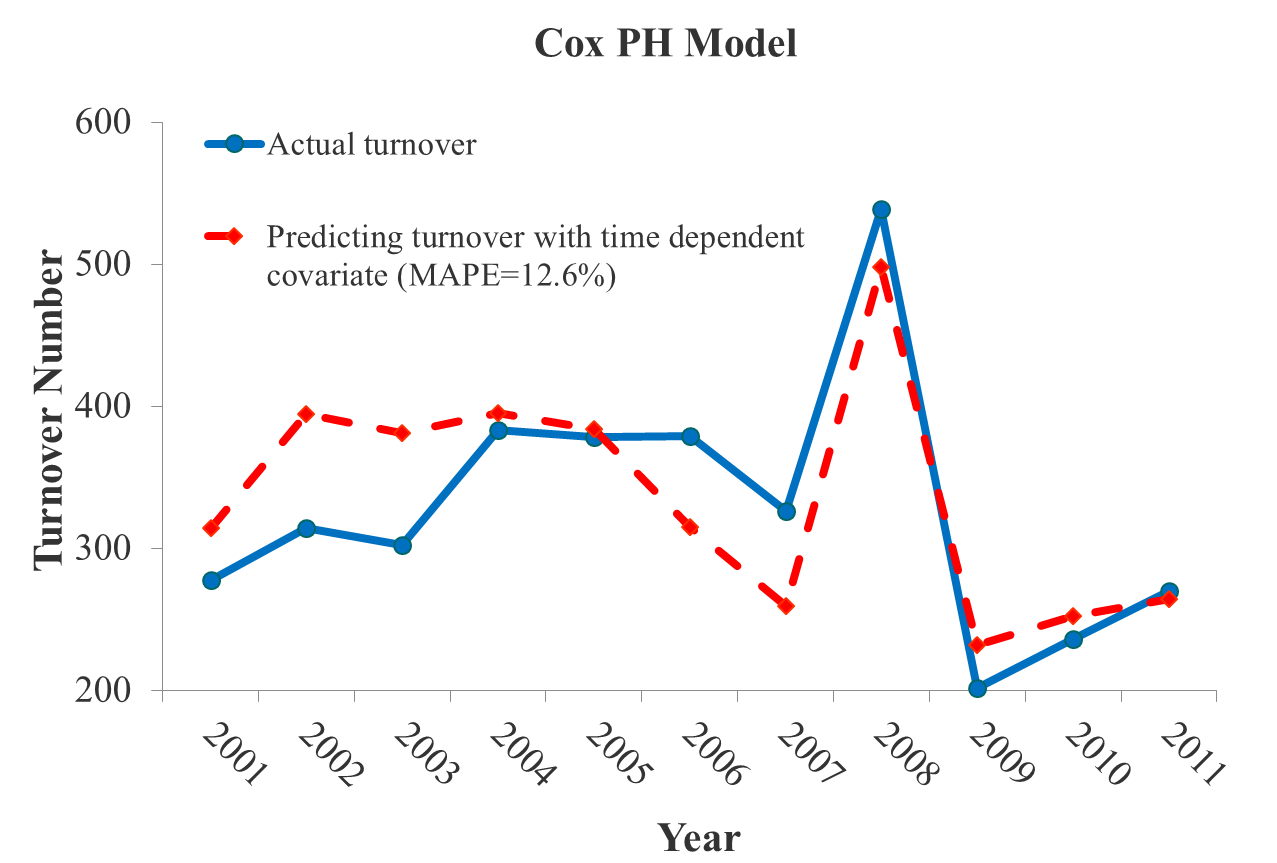
\includegraphics[width=5.5in]{Fig9.png}
	\caption{Actual vs. predicted turnover number for Cox PH model}
	\label{fig:9}
\end{figure}


%%%%%%%%%%%%%%%%%%%%%%%%%%%%
%%%%%%%%%%%%%%%%%%%%%%%%%%%%
%%%%%%%%%%%%%%%%%%%%%%%%%%%%
\subsection{Right censoring simulation result}
The right censoring simulation result shows Cox PH model coefficient estimate, baseline parameter estimates for Weibull distribution, and $-$log likelihood value for models with no censoring, 25\%, 50\%, and 75\% censoring proportion as shown in Table \ref{table:rightcensor}. The events in the second column of the table indicate total failure events in the dataset without including censoring, which is $events=\sum_{i=0}^{4000}{\delta_i}$ where $\delta$ is censor variable. The coefficients of age for all four models are all close to 0.025, but it is over estimates (0.026) when high proportion of censoring (75\%) in the dataset. The overestimation is also shown by the estimates of shape parameter: the estimated value (1.539) for model with 75\% censoring is greater than $\alpha=1.5$. It underestimates the shape parameters when the censoring proportion is 25\% and 50\%, respectively. The most close estimation of shape is when there is no censoring in the data. The $-$log likelihood values decrease from low percentage censoring to high percentage censoring. Because the scale parameter is generated by the formula, there is no actual value of scale parameter to compare. However, compared to the estimated value from no censoring (2.668), the model overestimates with 25\% censoring (2.779), get close with 50\% censoring (2.675) and underestimates with 75\% censoring (1.539). The estimates decrease when the percentage of censoring increases. Overall, the estimates are close to actual simulated value when the censoring proportion is close to 50\%. However, it over- or under-estimates the coefficients when the censoring proportion is 75\%. The phenomenon is also verified by plotting the actual and predicted failure number in the figure \ref{fig:7}.  The red line is the actual failure number simulated by Weibull distribution. The dark blue line is the predicted failure number for the model with 75\% censoring which is higher than all the other three lines for predicted failure number before time 3.75 and overlaid with the other three lines after 3.75. The gap between this line and the others three lines reaches the largest value around time 1. The other three lines represent the predicted failure number from the model with no censor, 25\% censoring, and 50\% censoring, respectively. They are too close to be distinguished in the figure. Therefore, the right censoring simulation shows that the Cox PH model performs well and the estimates are close to the actual values when the censoring proportion is close to 50\%, and it deteriorates when the censoring proportion is 75\%, causing the overestimation of the total failure number.
% Table generated by Excel2LaTeX from sheet 'Sheet2'
% Table generated by Excel2LaTeX from sheet 'Sheet1'
\begin{table}[htbp]
	\renewcommand{\arraystretch}{1.5}
	\small
	\centering
	\caption{Right censoring simulation statistics}
	\begin{tabular}{ccrrrc}
		\hline
		\multirow{2}[2]{*}{Models} & \multirow{2}[2]{*}{Events} & \multicolumn{3}{c}{Variable estimate} & \multirow{2}[2]{*}{$-$ loglikelihood} \\ \cline{3-5}
		
		&       & Age   & Scale & Shape &  \\\hline
		No Censor & 4000  & \multicolumn{1}{c}{0.024} & \multicolumn{1}{c}{2.668} & \multicolumn{1}{c}{1.494} & 4127.4 \\
		25\% Censored & 3000  & \multicolumn{1}{c}{0.025} & \multicolumn{1}{c}{2.779} & \multicolumn{1}{c}{1.480} & 3446.3 \\
		50\% Censored & 1999  & \multicolumn{1}{c}{0.024} & \multicolumn{1}{c}{2.675} & \multicolumn{1}{c}{1.487} & 2574.1 \\
		75\% Censored & 1000  & \multicolumn{1}{c}{0.026} & \multicolumn{1}{c}{2.643} & \multicolumn{1}{c}{1.539} & 1486.9 \\
		\hline
	\end{tabular}%
	\label{table:rightcensor}%
\end{table}%
\begin{landscape}
\begin{figure}[htbp]
	\centering
	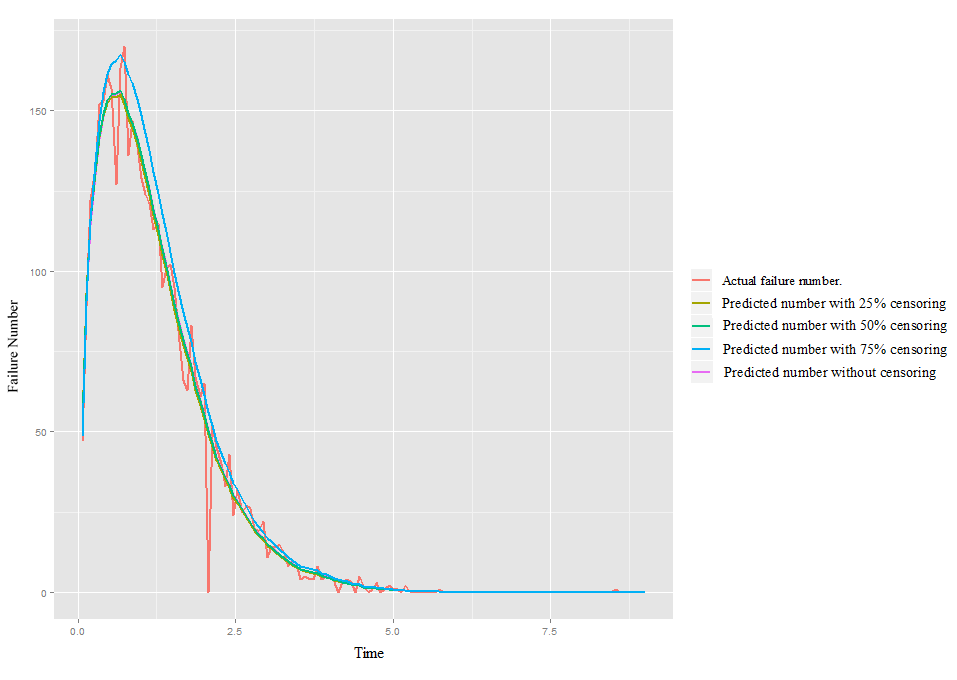
\includegraphics[width=9in]{Fig7}
	\caption{Actual vs. predicted failure number with various censoring}
	\label{fig:7}
\end{figure}
\end{landscape}
% % % % % % % % % % % % % % % % % % % % % % % % %
% % % %Left truncation result % % % % % % % % % % 
% % % % % % % % % % % % % % % % % % % % % % % % %
\subsection{Left truncation simulation results}
The left truncation bias simulation statistics for testing Cox PH model function shows coefficient estimate for age, baseline parameter estimates for scale and shape by Weibull distribution, $-$log likelihood value, and total predicted failure number for models with no left truncation, 25\%, 50\%, and 75\% left truncation proportion as shown in Table \ref{tab:lefttruncation}. The coefficients of age for all four models are all close to 0.025, even when high proportion of left truncation (75\%) in the dataset. However, the scale and shape parameter are over estimated, when the left truncation proportion is high: the estimated values for scale are 2.656, 2.620, 2.664, and 2.748 for no left truncation, 25\%, 50\%, and 75\%, respectively. The estimated values for shape are 1.483, 1.501, 1.504, and 1.539 for no left truncation, 25\%, 50\%, and 75\%, respectively. The estimation of the scale and shape for Weibull  distribution is close to simulation value when the left truncation portion is 25\% and 50\%. The model overestimates the parameters when left truncation proportion is 75\%, which is greater than $\alpha=1.5$. The last column is the summation of predicted failure number at each time point. They are close to actual failure number (4005, 2992) when left truncation proportion is 0\% and 25\%, respectively. When left truncation reaches to 50\% and 75\%, the failure number are around 50 more than the actual (2051 and 1059). However, the predicted failure number is smoothed and close to the actual one as shown in the figure \ref{fig:lefttruncation}. It is overestimates at the beginning of the time line when left truncation proportion is 50\% and 75\% as shown in figure \ref{fig:left50} and \ref{fig:left75}, where the dash lines are both higher than the solid lines at the beginning. 
Therefore, the left truncation simulation test shows that the Cox PH model performs well when the censoring proportion is less than 50\%, and it deteriorates when the truncation proportion goes high causing the overestimation of the total failure number.
\begin{table}[h!]
	\renewcommand{\arraystretch}{1.5}
	\small
	\centering
	\caption{Left truncation simulation statistics}
	\begin{tabular}{ccccccc}
		\hline
		\multirow{2}[4]{*}{Model} & \multirow{2}[4]{*}{Events} & \multicolumn{3}{c}{Variable Estimates} & \multirow{2}{3cm}{$-$ log.Likelihood} & \multirow{2}{3cm}{Predicted Total Failure No.}  \\
		\cline{3-5} % \cline{i-j} partial horizontal line beginning in column i and ending in column j		
				&       & Age   & Scale & Shape &  &\\				
		\hline
		No left Truncation & 4000  & 0.024 & 2.656 & 1.483 & 4167.8  &4005\\
		25\%  left Truncation & 3000  & 0.023 & 2.620  & 1.501 & 3041.2 & 2992\\
		50\%  left Truncation & 2000  & 0.023 & 2.664 & 1.504 & 1990.8 & 2051\\
		75\%  left Truncation & 1000  & 0.025 & 2.748 & 1.539 & 885.55 &2059\\
		\hline
		\end{tabular}%
	\label{tab:lefttruncation}%
\end{table}%
%negative loglikelihood value can be dropped. does not make sense.

\begin{figure}[h!]
	\centering
	\subfloat[No left truncation]{\label{fig:leftno}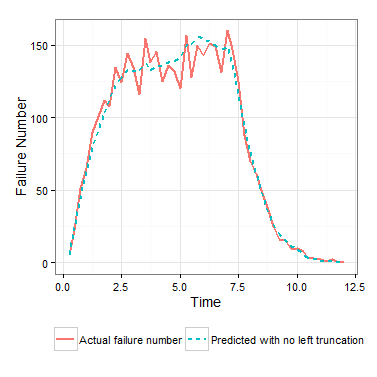
\includegraphics[width=2.75in]{notruncation.png}}
    \quad
	\subfloat[25\% left truncation]{\label{fig:left25}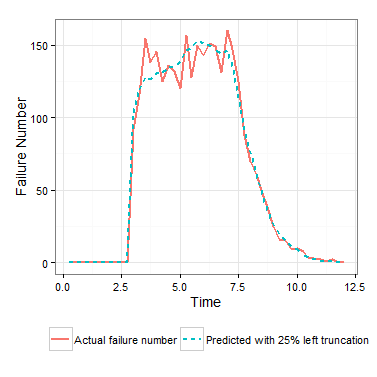
\includegraphics[width=2.75in]{25color.png}}
	\quad
	\subfloat[50\% left truncation]{\label{fig:left50}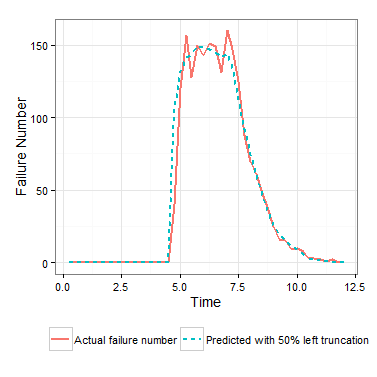
\includegraphics[width=2.75in]{50color.png}}
	\quad
	\subfloat[75\% left truncation]{\label{fig:left75}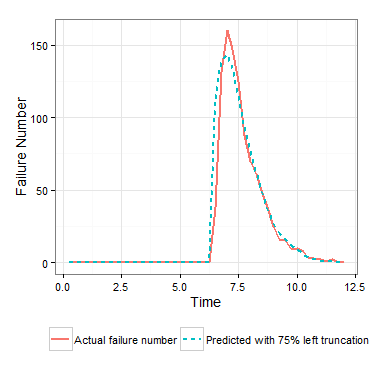
\includegraphics[width=2.75in]{75color.png}}
	\caption{Left truncation simulation results: actual vs. predicted failure number}
	\label{fig:lefttruncation}
\end{figure}
\subsection{Variable Selection}
The payroll is dropped from the variable list, because it is highly associated with Cocs as shown in table \ref{tab: freq1}. C and R are hourly payroll. E, M, and S are monthly payroll. G and T are weekly payroll. Only L and P have two levels of payroll, but L is mainly hourly payroll, and P is mainly monthly payroll. Their small parts are not reach 1\% of total employee number. Thus, the payroll is dropped from variable list.          
\begin{table}[htbp]
	\centering
	\small
	\renewcommand{\arraystretch}{1.5}
	\caption{ Table of Payroll by Cocs in percentage }
	\begin{tabular}{llllllllllll}
		\hline
		\multirow{2}[4]{*}{Payroll} & \multicolumn{10}{c}{Cocs} \\ \cline{2-11}
		
	
		& C     & E     & G     & L     & M     & P     & R     & S     & T     & Total \\ \hline
		H     & 14.27 & 0     & 0     & 8.78  & 0     & 0     & 6.75  & 0     & 0     & 29.79 \\
		M     & 0     & 16.45 & 0     & 0     & 16.01 & 20.66 & 0     & 2.38  & 0     & 55.50 \\
		W     & 0     & 0     & 6.27  & 0.35  & 0     & 0.01  & 0     & 0     & 8.08  & 14.71 \\
		Total & 14.27 & 16.45 & 6.27  & 9.12  & 16.01 & 20.67 & 6.75  & 2.38  & 8.08  & 100 \\
		\hline
	\end{tabular}%
	\label{tab: freq1}%
\end{table}%


